%for a more compact document, add the option openany to avoid
%starting all chapters on odd numbered pages
\documentclass[12pt]{cmuthesis}

% This is a template for a CMU thesis.
% The source for this is pulled from a variety of sources and people.
% Here's a partial list of people who may or may have not contributed:
%
%        bnoble   = Brian Noble
%        caruana  = Rich Caruana
%        colohan  = Chris Colohan
%        jab      = Justin Boyan
%        josullvn = Joseph O'Sullivan
%        jrs      = Jonathan Shewchuk
%        kosak    = Corey Kosak
%        mjz      = Matt Zekauskas (mattz@cs)
%        pdinda   = Peter Dinda
%        pfr      = Patrick Riley
%        dkoes    = David Koes

% some useful packages
\usepackage{times}
\usepackage{fullpage}
\usepackage{graphicx}
\usepackage{amsmath}
\usepackage[numbers,sort]{natbib}
\usepackage[backref,pageanchor=true,plainpages=false, pdfpagelabels, bookmarks,bookmarksnumbered,
%pdfborder=0 0 0,  %removes outlines around hyper links in online display
]{hyperref}
\usepackage{subfigure}
\usepackage{braket}

% Approximately 1" margins, more space on binding side
%\usepackage[letterpaper,twoside,vscale=.8,hscale=.75,nomarginpar]{geometry}
%for general printing (not binding)
\usepackage[letterpaper,twoside,vscale=.8,hscale=.75,nomarginpar,hmarginratio=1:1]{geometry}

\setcounter{secnumdepth}{3}
\setcounter{tocdepth}{3}

% Provides a draft mark at the top of the document.
\draftstamp{\today}{DRAFT}

\usepackage{cleveref}

\begin {document}
\frontmatter

%initialize page style, so contents come out right (see bot) -mjz
\pagestyle{empty}

\title{ %% {\it \huge Thesis Proposal}\\
{\bf Benchmarking OODA Loop of an Edge-Enabled Autonomous Drone System with On-Board Compute}}
\author{Aditya Chanana}
\date{December 18}
\Year{2024}
\trnumber{}

\committee{
Mahadev Satyanarayanan, Chair \\
Padmanabhan Pillai\\
}

\support{}
\disclaimer{}

% copyright notice generated automatically from Year and author.
% permission added if \permission{} given.

\keywords{edge computing, drones, mobile networks, latency, bandwidth, edge-native applications, computer vision, machine learning}

\maketitle

\begin{dedication}
“Science, my lad, is made up of mistakes, but they are mistakes which it is useful to make, because they lead little by little to the truth.” Jules Verne
\end{dedication}

\pagestyle{plain} % for toc, was empty

%% Obviously, it's probably a good idea to break the various sections of your thesis
%% into different files and input them into this file...

\begin{abstract}

    The "Observe, Orient, Decide, Act" (OODA) loop encapsulates the agility of
    cyber-physical or cyber-human systems that depend on continuous iterations
    of these steps. Systems with faster OODA loops react more quickly to
    changes in their environment. This work extends the SteelEagle
    cloudlet-based autonomous drone system to utilize onboard computational
    abilities. We bechmark the OODA loop of the new setup and identify
    opportunities for optimization. We show how to combine the use of onboard
    computational abilities, for tasks that benefit immensely from a faster OODA loop,
    and offloading, for tasks that are more computationally expensive, leading
    to an optimal system that excels in real-time computer visions tasks.

\end{abstract}

\begin{acknowledgments}
Dave Eckhardt
\end{acknowledgments}



\tableofcontents
\listoffigures

\listoftables

\mainmatter

%% Double space document for easy review:
%\renewcommand{\baselinestretch}{1.66}\normalsize

% The other requirements Catherine has:
%
%  - avoid large margins.  She wants the thesis to use fewer pages,
%    especially if it requires colour printing.
%
%  - The thesis should be formatted for double-sided printing.  This
%    means that all chapters, acknowledgements, table of contents, etc.
%    should start on odd numbered (right facing) pages.
%
%  - You need to use the department standard tech report title page.  I
%    have tried to ensure that the title page here conforms to this
%    standard.
%
%  - Use a nice serif font, such as Times Roman.  Sans serif looks bad.
%
% Other than that, just make it look good...

\chapter{Introduction}
% Goal : 5-10 page talk before the talk
% maybe not 10 pages, but providing a general overview of the paper is the goal here
\section{Motivation}
\label{sec:motivation}
Mobile devices, such as smartphones and smartwatches, have a key limitation---a
limited battery life which allows them to operate for finite periods before
requiring recharging.  Resource-intensive applications, such as those involving
augmented reality or deep learning inference, exacerbate the situation by
accelerating battery depletion.  Consequently, a mobile device cannot match the
sustained performance and resource capacity of stationary computers, which are
free from the requirements of mobility. Mobile devices will always lag behind
static devices in computational ability because of their size and weight
constraints \cite{satya2014}. Increased computational ability, at the same
level of hardware efficiency, demands higher energy consumption. This requires
larger batteries to preserve operating time, thereby increasing weight and
size---which are undesirable for mobile devices.
\Cref{tab:mobility-constraints} shows how mobile devices have lagged behind
servers in computational power over a period of 25 years. This limitation has
been referred to as the ``mobile penalty'', the cost for reduction in
performance required to adhere to mobility constraints
\cite{satya-edge-native}.

\begin{table}[htbp]
    \centering
    \begin{tabular}{@{}lllll}
        \toprule & \multicolumn{2}{c}{\textbf{Typical Server}} & \multicolumn{2}{c}{\textbf{Typical Mobile Device}}\\\midrule
        \textbf{Year} & \textbf{Processor} & \textbf{Speed} & \textbf{Device} & \textbf{Speed}\\\midrule
        1997 & Intel Pentium II & 266 MHz & Palm Pilot & 16 MHz\\
        2002 & Intel Itanium & 1 GHz & Blackberry 5810 & 133 MHz\\
        2007 & Intel Core 2 Quad Q6600 & 2.4 GHz x 4 & Apple iPhone & 412 MHz\\
        2012 & Intel Xeon E5-2690 & 3.8 GHz x 8 & Samsung Galaxy S3 & 1.4 GHz x 4\\
        2017 & Intel Xeon Platinum 8180 & 3.8 GHz x 28 & Google Pixel 2 & 2.35 GHz x 4,\\
             &&&& 1.9 GHz x 4\\
        2022 & AMD EPYC 9654 & 3.7 GHz x 96 & Samsung Galaxy S22 Ultra & 3 GHz x 1,\\
             &&&& 2.5 GHz x 3,\\
             &&&& 1.8 Ghz x 4\\
        \bottomrule
    \end{tabular}
    \begin{captext}
        *While processor efficiency depends on more factors than processor frequency, such as instructions per cycle, it provides a good first-order approximation.
    \end{captext}
    \caption{The Mobility Penalty Over a Period of 25 Years (Adapted from Chen \cite{zchenthesis}, Flinn \cite{flinn2012cyber})}
    \label{tab:mobility-constraints}
\end{table}

Unmanned aerial vehicles (UAVs), or drones, which spend most of their energy on
flight, are particularly affected by this limitation. Larger batteries required
to sustain intensive on-drone computation increases drone weight.  Increased
drone weight leads to an upwards spiral in weight as larger rotors and more
powerful motors are needed to achieve the same amount of lift.  This requires
even larger batteries which, in turn, may require a more reinforced aircraft
structure, and so on. How, then, can we enable mobile devices to do more given
the mobility constraints they are subject to? Advancements in hardware
efficiency provide one possible way forward, but these advancements are slow
and far between. It turns out that there is a way to "cheat" that enables
mobile devices to do more today, leveraging static infrastructure to overcome
the mobility penalty, known as offloading.

A significant body of work in the field of mobile computing has utilized cloud
or cloudlet offloading techniques to address the inherent resource poverty of
mobile devices \cite{satya1996,satya2009}. Cloudlet offload allows mobile
devices to remotely execute computationally expensive tasks on cloudlets that
do not need to be light or small. This allows mobile devices to retain their
low weight and small size, but possess superior computational abilities.

Drones are an excellent category of mobile devices to study because of their
wide range of useful applications as well as their design requirements which
take mobility constraints to the extreme.  We benchmark an autonomous drone
system that leverages offloading techniques to overcome the computational
limitations of consumer-grade drones. We identify its limitations and evaluate
its performance to understand the areas that future work should focus on to
enable more capable drones that can have a wider variety of application.

\section{Overview}
\label{sec:overview}

SteelEagle \cite{bala2024} is an autonomous drone system that leverages
offloading.  Its main tenet is the use of commerical-off-the-shelf (COTS)
drones, which are readily available at low cost but typically have minimal to
no on-board computational resoures.  Utilizing cloudlet offload, SteelEagle
enables COTS drones to perform much more intelligent tasks than what they were
designed for, and exhibit autonomous capabilities typically only found in
larger, more expensive drones.  SteelEagle focuses on active vision tasks which
require the ability to perform live video analytics during flight to determine
the next course of action. SteelEagle drones relay their camera video stream
over a commercial cellular network to a nearby on-ground edge server, a
cloudlet, which runs a computationally expensive pipeline involving neural
networks (\cref{fig:steeleagle-drone-arch}) to perform tasks such as monocular
camera depth perception.  This processing of the raw drone sensor stream allows
obtaining higher level semantic information about the drone's physical
environment. In the case of depth perception, we could infer obstacles that
present the danger of a collision. The drone can then be sent piloting commands
to react, perhaps to actuate to avoid an impending collision.

\begin{figure}[htbp]
\centerline{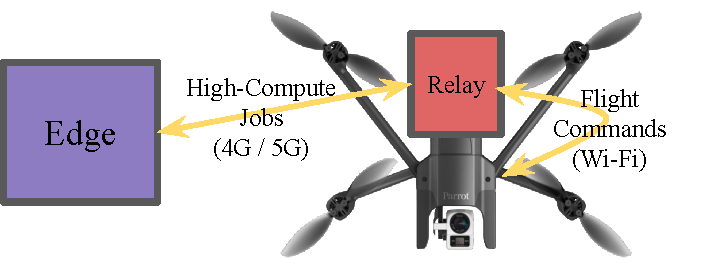
\includegraphics[width = .6\textwidth]{figs/steeleagle-drone-arch-cropped.pdf}}
\caption{Cloudlet Offload in SteelEagle}
\label{fig:steeleagle-drone-arch}
\end{figure}

An important consideration for SteelEagle is the agility of the resulting
system.  How quickly can a drone respond to a change in its environment? The
end-to-end latency of the entire execution pipeline, including sensing,
offloading, inferencing, decision making, and actuation, defines the agility. A
high end-to-end latency can severely handicap the drone---it must fly at a
higher altitude or at lower speeds to be safe if it takes a long time to
identify obstacles and actuate to avoid them. Drone flight at a higher altitude
precludes close observation, and lower speeds make missions take longer,
limiting the capabilities of the drone. Search and rescue missions in forests,
and missions to aid law enforcement operations in dense cities, for instance,
must fly at low altitudes while avoiding obstacles in the environment that
present a collision risk---trees branches, streetlight poles, utility wires,
and buildings---without impacting mission speed. Unless we can achieve high
agility, SteelEagle drones will struggle to perform these missions well.  Since
these missions are one of the most compelling use cases for autonomous drones,
benchmarking the end-to-end pipeline to determine latency bottlenecks and
identifying opportunities for latency optimization is a very worthy pursuit.

SteelEagle drones currently perform no onboard computation---they are
controlled exclusively over the network.  While this strategy allows treating
consumer-grade non-programmable drones as black boxes, it presents severe
limitations. First, SteelEagle drones struggle in areas with unreliable cell
service and are completely inoperable in regions without cellular coverage.
Second, cloudlet offload imposes an upper bound on drone agility as it adds the
cost of a round-trip latency to a cloudlet. As originally envisioned, cloudlets
are differentiated from clouds because of their network proximity, which allows
application end-to-end response time to be just a few milliseconds. In
practice, the usage of commerical cellular networks for offload to the cloudlet
increases this latency to tens of milliseconds. This limits the agility of the
drone, as the reaction time is at least the round-trip time to the cloudlet.

This thesis performs a comprehensive benchmarking of the SteelEagle system,
revealing the current system bottlenecks and identifying opportunities for
optimization. In recent years, domain-specific system-on-a-chip devices have
become available that provide substantial energy-efficient on-board
computational resources through the inclusion of hardware accelerators in the
chip design. These chips can decode the video stream generated by the drone and
perform analytics using TensorFlow Lite models, and often include 5G and Wi-Fi
connectivity. Using such a chip as a payload on SteelEagle drones allows us to
continue treating the drone as a black box, but employ new cloudlet offload
tactics that result in tighter OODA loops for use cases that can utilize the
hardware accelerators, while retaining the generality offered by cloudlet
offload. We explore the use of onboard computation to mitigate the limitations
of SteelEagle, and explore the resulting impact on drone agility.

\section{Contributions}

The contributions of this thesis include
\begin{itemize}
  \item A discussion of efforts to optimize SteelEagle that yielded a two-fold
      improvement in drone-to-cloudlet latency
  \item A mapping of the SteelEagle pipeline to the OODA loop framework
  \item An analysis of the SteelEagle pipeline's performance from a latency
      and bandwidth perspective
  \item An evaluation of the use of an onboard computation device to improve
      SteelEagle performance and alleviate its limitations
\end{itemize}

\section{Organization}
\Cref{ch:background} provides a detailed background on edge computing and the
SteelEagle autonomous drone system. \Cref{ch:uav-primer} describes the history
of drones and their development over time. We discuss the applications that
drones are used in today, as well as the capabilities of today's drones.  We
also discuss what autonomy means for drones. In
\cref{ch:optimizing-steeleagle}, we describe our experimental setup for
measuring the latency of the SteelEagle system. We include measurements which
provided the insight needed to optimize SteelEagle, allowing for a two-fold
improvement in SteelEagle's drone-to-cloudlet latency. In \cref{ch:voxl}, we
explore the use of an onboard computation device called the Modal AI VOXL to
augment SteelEagle. We conclude with \cref{ch:conclusion}, presenting
concluding remarks and providing a road map for future work.


\begin{comment}
The "Observe, Orient, Decide, Act" (OODA) loop framework devised by military
strategist John R. Boyd provides a framework to structure our investigation
into the end-to-end latency of SteelEagle. According to Boyd, decision-making
happens in a continuous iteration of these steps. Boyd attributed the faster
OODA loop of U.S. pilots flyng F-86s, because of the bubble-shaped canopy
offering better visibility and hydraulic controls that allowed for easier
switching between manoeuvres, as the reason the slower F-86s fared better than
the North Korean MiG-15s during the Korean War \cite{morton1995}. A system with
a tighter OODA loop corresponds to a more agile drone. Instead of measuring
just the overall system latency, performing a break down of the latency across
the OODA steps provides more insight into system latency bottlenecks.
\end{comment}

\chapter{Benchmarks}

hello



\chapter{Section 1}

We have discussed many things.
But, it is unclear we have really discussed the nature of them.

\section{More things}

\subsection{Moore things}

We can even put a picture in here, which is harder than it looks.

\begin{figure}[htbp]
\centerline{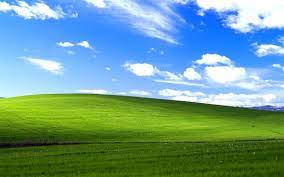
\includegraphics[width = .85\textwidth]{Unknown.jpeg}}
\caption{Something}
\label{fig}
\end{figure}
\chapter{Section 2}

We have derived the basics of things.
Now let us look at the things themselves.

\section{The things are alive}

This is a table.

\begin{table}[h!]
\centering
\begin{tabular}{ |p{1cm}||p{2cm}|p{2cm}|p{5cm}|p{3cm}| }
 \hline
 \multicolumn{5}{|c|}{Table of things that are alive} \\
 \hline
 T & H & i & N & G \\
 \hline
 Alps   & 0  & 5 &  e & hovercraft\\
 16   & dog  & 5 &  e & 80\\
 32   & 0  & pangolin &  l & 210\\
 M   & 0  & 5 &  s & 810\\
 \hline
\end{tabular}
\caption{Table to test captions and labels}
\label{table:1}
\end{table}
\chapter{Conclusion and Future Work}
\section{Conclusion}
Tell me
\section{Future Work}



%\appendix
%\include{appendix}

\backmatter
%\renewcommand{\baselinestretch}{1.0}\normalsize

% By default \bibsection is \chapter*, but we really want this to show
% up in the table of contents and pdf bookmarks.
\renewcommand{\bibsection}{\chapter{\bibname}}
%\newcommand{\bibpreamble}{This text goes between the ``Bibliography''
%  header and the actual list of references}
\bibliographystyle{plainnat}
\bibliography{register} %your bib file

\begin{thebibliography}{00}

\bibitem{thing} thing

\end{thebibliography}

\end{document}
